\documentclass[11pt,a4paper]{article}
\usepackage[margin=2.5cm]{geometry}
\usepackage{parskip}
\usepackage{microtype}
\usepackage{amsmath}
\usepackage{booktabs}
\usepackage{enumitem}
\usepackage{listings}
\usepackage{tikz}
\usetikzlibrary{arrows.meta}
\usepackage[hidelinks]{hyperref}

\lstset{
  basicstyle=\ttfamily\footnotesize,
  frame=single,
  framerule=0.4pt,
  breaklines=true,
  breakatwhitespace=true,
  postbreak=\mbox{\hspace{2em}},
  columns=fullflexible,
  keepspaces=true,
  showstringspaces=false,
  keywordstyle={},
  aboveskip=0.9em,
  belowskip=0.9em
}

\title{GradeTrack: A Student Performance and Attendance Tracker}
\author{Aditya Maiti}
\date{}

\begin{document}
\maketitle

\section{Introduction}

GradeTrack is a web application for tracking student marks and attendance. It serves three roles. Teachers record graded work and attendance for the classes they own. Students see their own results and trends. Administrators manage accounts and watch performance across the whole school.

The system is a Go HTTP API over MySQL with a React single-page frontend. This report describes the design decisions behind it and what each decision caused in the code. The data model changed once during development. The first model stored marks as flat rows and failed in use. Sections \ref{sec:v1} and \ref{sec:v2} present that failure and the correction honestly, because most of what the finished system can do follows from the corrected model.

The report moves in the order the problems appeared: roles and access control first, then the data model, then the reporting and visualization the model made possible, then the hardening work, and finally the known limitations.

\section{System overview}

The backend is Go 1.25 with the Gin router, the sqlx database library, and MySQL 8. The frontend is React 18, built with Vite, using react-router for navigation and Recharts for charts. The two sides talk only through a JSON API under \texttt{/api}. The server reads its configuration from environment variables and refuses to start without a \texttt{JWT\_SECRET}.

The backend follows a small layering rule. Handlers parse and validate requests, then call the \texttt{db} package. The \texttt{db} package owns every SQL statement, one file per table. The \texttt{models} package holds plain structs that match rows. There is no ORM. sqlx scans query results into the structs and the SQL stays visible in the source. This is an ordinary choice, but it matters later: the performance report is a single hand-written query, and section \ref{sec:perf} can show it directly.

The database schema lives in one \texttt{schema.sql} file that drops and recreates every table. A \texttt{seed.sql} file loads a demo school: one admin, two teachers, seven students, two classes, ten assessments, and 43 mark rows. The worked examples in this report use these seed numbers.

\section{Authentication}

Every later decision depends on knowing who is calling and what their role is. So authentication came first, and it puts the role inside the token.

A successful login returns a JWT signed with HS256. The token carries two custom claims, \texttt{user\_id} and \texttt{role}, next to the registered claims. It expires after eight hours and pins an issuer and an audience. Because the role travels in the token, no handler ever queries the database to find out what the caller is allowed to be. The \texttt{AuthRequired} middleware verifies the token once and stores \texttt{user\_id} and \texttt{role} in the request context. A second middleware, \texttt{RequireRole}, reads the stored role and rejects the request with 403 if it is not in the allowed list.

Passwords are hashed with bcrypt at cost 12. Password length is bounded to 8 to 72 characters; 72 is bcrypt's input limit. If a stored hash was created at a lower cost, a successful login transparently re-hashes the password at the current cost.

Account creation is split by role. The public registration endpoint creates student accounts only; any role field in the request body is ignored. Teacher and admin accounts are created by an admin. Each such account gets a random 12-character temporary password, returned exactly once in the API response, and a \texttt{must\_change\_password} flag. The frontend redirects a flagged user to the password change page before anything else. Admins can also reset any account to a fresh temporary password with the same forced change.

Accounts are deactivated, never deleted. An \texttt{is\_active} flag blocks login with 403 but keeps every mark and attendance row. The seed data includes a student who left mid-term: the account is inactive, and the Term 1 history is still there for reports.

\section{Route protection}

The role claim says what kind of user is calling. It does not say whether that user may act on one specific class or mark. That second question is ownership. It is easy to get wrong when every handler checks it by hand.

GradeTrack centralizes ownership in one file of scoping middleware. Each middleware resolves the \texttt{:id} route parameter to its row, walks up to the owning class, checks the caller against that class, and stores the loaded rows in the request context. There are three levels of check. Class access allows an admin, the owning teacher, or an enrolled student. Class manager allows an admin or the owning teacher. Class owner allows only the owning teacher; recording marks and attendance is deliberately not an admin power. Every route with an \texttt{:id} parameter is wrapped by exactly one scoping middleware or by the admin gate, which makes the protection auditable by reading the routing table:

\begin{lstlisting}[language=Go]
auth.POST("/classes/:id/assessments", RequireClassOwner(), CreateAssessment)
auth.GET("/classes/:id/assessments", RequireClassAccess(), ListAssessments)
auth.PUT("/assessments/:id", RequireAssessmentOwner(), UpdateAssessment)
auth.DELETE("/assessments/:id", RequireAssessmentOwner(), DeleteAssessment)

auth.POST("/assessments/:id/marks", RequireAssessmentOwner(), RecordMark)
auth.POST("/assessments/:id/scores", RequireAssessmentOwner(), BulkScores)
auth.GET("/classes/:id/marks", RequireClassAccess(), ListMarks)
auth.PUT("/marks/:id", RequireMarkOwner(), UpdateMark)
auth.DELETE("/marks/:id", RequireMarkOwner(), DeleteMark)
\end{lstlisting}

Notice that every line pairs a route with exactly one guard, and that the guard name states the required relationship. A mark is reached through its assessment, so \texttt{RequireMarkOwner} loads the mark, then the assessment's class, then compares the class teacher to the caller. Handlers start with the row already loaded and already authorized.

Ownership is the first layer. The second layer is row narrowing inside list handlers. Marks, attendance, and performance listings accept any enrolled student, but when the caller's role is student, the handler restricts the query to that student's own rows. A student can never read a classmate's scores, even inside a class they belong to.

\section{The first data model}
\label{sec:v1}

The first version stored marks as flat rows. Each row carried \texttt{class\_id}, \texttt{student\_id}, a free-text \texttt{title}, a \texttt{score}, and a \texttt{max\_score}. A CHECK constraint required the score to be present and within range.

This model worked for its first job, entering one mark for one student. It failed as soon as the marks were used together. Three problems appeared.

First, the graded item had no identity of its own. ``Quiz 1'' for a class of 25 students was 25 copies of the title and the maximum score. Renaming the quiz or correcting its maximum meant updating every copy, and one typo in one row silently split the quiz into two different items in every report.

Second, there was nowhere to put a term or a category. Averages could only be computed over all marks at once. Term filtering and an assignment-versus-exam breakdown had no column to filter on.

Third, a missing score could not be recorded. The score column was NOT NULL and the constraint forbade anything outside the range. A student who skipped a quiz either got no row at all, which looks identical to a mark not yet entered, or got a zero, which is wrong because a zero is an earned grade.

\section{Data model revision}
\label{sec:v2}

The fix was to give the graded item its own table. This was a correction of a design mistake, not a planned migration; the flat model only revealed its problems once real class data went through it.

An \texttt{assessments} row holds what the flat rows had been duplicating: the class, the title, a category (\texttt{assignment}, \texttt{quiz}, or \texttt{exam}), a term, and the maximum score. A mark shrinks to a score attached to one assessment and one student, with a unique key on the pair. The score column becomes nullable, and NULL now means exactly one thing: the mark was recorded and the student has no score, distinct both from zero and from an absent row.

\begin{figure}[htbp]
\centering
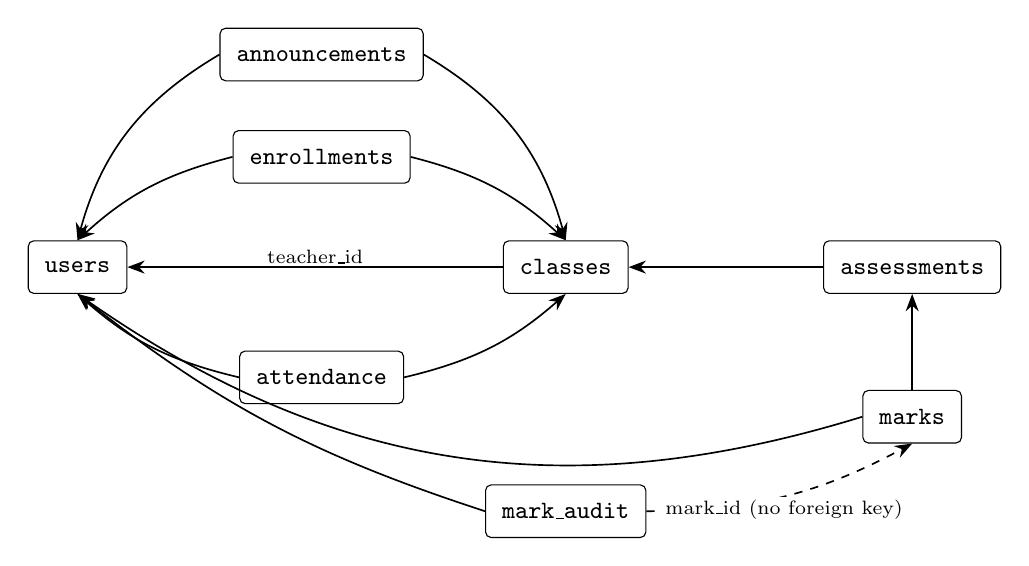
\begin{tikzpicture}[
  tbl/.style={draw, rounded corners=2pt, font=\small\ttfamily, minimum height=1.9em, inner sep=6pt},
  fk/.style={-{Stealth[length=2.2mm]}, semithick},
  lbl/.style={draw=none, fill=white, font=\scriptsize, inner sep=1pt}
]
\node[tbl] (users)   at (0,0)      {users};
\node[tbl] (classes) at (6.2,0)    {classes};
\node[tbl] (enroll)  at (3.1,1.4)  {enrollments};
\node[tbl] (ann)     at (3.1,2.7)  {announcements};
\node[tbl] (att)     at (3.1,-1.4) {attendance};
\node[tbl] (asm)     at (10.6,0)   {assessments};
\node[tbl] (marks)   at (10.6,-1.9){marks};
\node[tbl] (audit)   at (6.2,-3.1) {mark\_audit};

\draw[fk] (classes) -- node[lbl, above]{teacher\_id} (users);
\draw[fk] (enroll.west)  to[bend right=14] (users.north);
\draw[fk] (enroll.east)  to[bend left=14]  (classes.north);
\draw[fk] (ann.west)     to[bend right=22] (users.north);
\draw[fk] (ann.east)     to[bend left=22]  (classes.north);
\draw[fk] (att.west)     to[bend left=14]  (users.south);
\draw[fk] (att.east)     to[bend right=14] (classes.south);
\draw[fk] (asm) -- (classes);
\draw[fk] (marks) -- (asm);
\draw[fk] (marks.west)   to[bend left=26]  (users.south);
\draw[fk] (audit.west)   to[bend left=10]  (users.south);
\draw[fk, dashed] (audit.east) to[bend right=14] node[lbl, below]{mark\_id (no foreign key)} (marks.south);
\end{tikzpicture}
\caption{Final schema. Arrows point from a foreign key to the referenced table. The dashed reference from \texttt{mark\_audit} to \texttt{marks} is deliberately not a foreign key, so audit history survives a mark's deletion.}
\label{fig:schema}
\end{figure}

Figure \ref{fig:schema} shows the resulting schema. Each consequence of the split can be traced to one report feature.

The title and maximum score now live in one row. Renaming an assessment is one update. Lowering a maximum is guarded: the update is rejected if any recorded score would exceed the new maximum.

Terms and categories are plain columns on the assessment. Term filtering becomes a WHERE clause, and category breakdowns become a GROUP BY. Neither needed new storage.

The NULL score changes what averages mean. Averages are computed only over scored marks, and missing marks are counted separately. The seed data shows why this matters. Diya Patel has four scored marks in Algebra II and one missing quiz. Her average over the scored marks is 83.75\%. If the missing quiz were stored as a zero, the same column of numbers would read 67\%. The report shows 83.75\% with a missing count of 1, which is the honest version of both facts.

\section{Score entry}

With assessments in place, score entry could match how teachers actually grade: one assessment at a time, whole class at once.

The API has two write paths. A single-score endpoint records or overwrites one student's score on an assessment. A bulk endpoint accepts the whole roster for one assessment as a JSON array of entries, each holding a \texttt{student\_id} and a \texttt{score}, where a null score records a missing mark. The handler validates before anything is written: between 1 and 500 entries, no duplicate student ids, every student enrolled in the class, every score between zero and the assessment's maximum or null.

The bulk write is one transaction. Either every score lands or none do, so a failure halfway through a class of 30 cannot leave 15 students graded:

\begin{lstlisting}[language=Go]
func BulkUpsertMarks(assessmentID int64, entries []ScoreEntry, changedBy int64) error {
    tx, err := DB.Beginx()
    if err != nil {
        return err
    }
    defer tx.Rollback()
    // existing scores are read FOR UPDATE into prev, keyed by student (elided)
    for _, e := range entries {
        if _, err := tx.Exec(`INSERT INTO marks (assessment_id, student_id, score)
            VALUES (?, ?, ?) ON DUPLICATE KEY UPDATE score = VALUES(score)`,
            assessmentID, e.StudentID, e.Score); err != nil {
            return err
        }
        // entries that change a previous score append to mark_audit (elided)
    }
    return tx.Commit()
}
\end{lstlisting}

Notice the shape rather than the elided details. The upsert leans on the unique key over \texttt{(assessment\_id, student\_id)}: re-submitting a roster overwrites earlier scores instead of duplicating rows. The previous scores are read with a row lock inside the same transaction, both to make the diff safe under concurrency and to feed the audit rows described in section \ref{sec:hardening}. The deferred \texttt{Rollback} is a no-op after a successful commit and undoes everything on any early return.

Attendance entry follows the same pattern one level up: one date, the whole roster, present or absent per student, validated the same way, with re-submission of a date overwriting that day's statuses. Future dates are rejected.

\section{Performance aggregation}
\label{sec:perf}

Scores are stored against assessments, not as flat marks. The class performance report can therefore be one SQL query that normalizes each mark by its own maximum. A mark's percentage is $100 \times \textit{score} / \textit{max\_score}$, and a student's average is the mean of those percentages. Each mark carries equal weight regardless of its maximum, so a 10-point quiz counts as much as a 100-point exam. That is a deliberate, simple choice; weighted terms would need a weight column and are listed as future work.

The query joins two pre-aggregated subqueries onto the class roster, one for marks and one for attendance. Aggregating first matters. Joining the raw marks and attendance tables directly onto the roster would pair every mark row with every attendance row for the same student and inflate every SUM. The marks side looks like this:

\begin{lstlisting}[language=SQL]
SELECT u.id AS student_id, u.name, m.average_pct,
       COALESCE(m.mark_count, 0) AS mark_count,
       COALESCE(m.missing_count, 0) AS missing_count
FROM enrollments e
JOIN users u ON u.id = e.student_id
LEFT JOIN (
    SELECT mk.student_id, COUNT(mk.score) AS mark_count,
           SUM(mk.score IS NULL) AS missing_count,
           ROUND(AVG(mk.score / asm.max_score * 100), 2) AS average_pct
    FROM marks mk JOIN assessments asm ON asm.id = mk.assessment_id
    WHERE asm.class_id = ? AND (? = '' OR asm.term = ?)
    GROUP BY mk.student_id
) m ON m.student_id = u.id
WHERE e.class_id = ? AND (? = 0 OR u.id = ?)
\end{lstlisting}

Two details in the excerpt carry the design. \texttt{COUNT} and \texttt{AVG} skip NULL scores, while \texttt{SUM(mk.score IS NULL)} counts exactly the missing ones, so a missing mark never drags an average down and is never silently dropped either. And the repeated \texttt{(? = ...\ OR ...)} pattern makes the term filter and the student filter optional inside one prepared statement: passing an empty term includes every assessment, and passing student id 0 returns the whole roster. One query serves the teacher's full-class view, the student's own row, and every term filter.

A second query attaches per-category averages to each row, grouped by assessment category. A school-wide variant of the same aggregation feeds the admin overview: it averages each active student's per-class average, computes total attendance, and counts students at risk.

\section{Visualization}

The visualization layer exists to answer questions that the raw tables do not: who needs help, whether absence explains low scores, and whether things are getting better. The server returns aggregates and raw lists; the charts and their derived series are computed in the browser. This avoids one endpoint per chart and keeps chart changes out of the API.

The frontend is organized around one page per class with five tabs: a stream of announcements, marks, attendance, performance, and the roster. Which tabs allow editing follows the caller's role, mirroring the server-side guards. Each role also has its own dashboard listing its classes or, for the admin, the school.

One rule spans the whole layer. A student is at risk when their average falls below 40\% or their attendance falls below 75\%. The same thresholds appear in the client chart code and in the admin overview SQL, so a student flagged in a teacher's chart is the same student counted on the admin dashboard.

Teachers get four main views per class. A sorted bar chart of average score by student, with a dashed line at the 40\% threshold, answers who needs help right now. A scatter of attendance against average answers whether low scores go with absence. In the seed data it places Fiona Chen at a 37\% average and 30\% attendance, flagged on both counts. A per-assessment histogram of score buckets, with the missing count alongside, answers whether one assessment was unusually hard or easy. A term comparison shows the class average per term, computed by averaging each student first so one student with many marks cannot dominate the class figure. A per-session attendance line, a per-student heatmap with a current-streak count, and a grid of per-student sparklines fill in the session-level and trend detail.

Students get the same data narrowed to themselves. A marks-over-time line shows each mark as a percentage of its maximum. Category bars compare their assignment, quiz, and exam averages. A chart across their classes compares averages per class, and a personal term comparison shows whether their own averages are rising or falling.

Admins get school-level tiles for student, teacher, and class counts, the school average, school attendance, and the at-risk count, backed by a per-class chart of average and attendance and a per-teacher load chart of classes and students taught.

\section{Administration and class tools}

A tracker is only useful once the accounts and rosters are in it, and typing in 200 student accounts one at a time is not realistic. This section covers the tooling around that, and one deliberate contrast with the score entry design.

Admins can import students in bulk. The browser parses an uploaded CSV file with a small hand-written parser and sends the rows as JSON, up to 500 at a time. The server validates each row and answers with a per-row status: created, duplicate email, duplicate roll number, or invalid. All created accounts share one generated temporary password, with the forced password change described in section 3.

The import is intentionally not transactional, which is the opposite of the bulk score write. Scores for one assessment belong together, so a partial write is harmful and the transaction rejects it. Imported accounts are independent of each other, so a file with three bad rows should still create the other 197 and name the three that failed. The correct unit of failure differs between the two features, and each endpoint implements its own.

Class marks and the attendance register can be exported as CSV files, generated in the browser from data already loaded, with proper quoting and a byte-order mark so spreadsheet programs open them cleanly. The attendance tab includes a monthly register view: students as rows, the month's session dates as columns, with per-day totals, derived entirely from the raw attendance list.

Two smaller tools round this out. The admin user list supports a single search box that matches name, email, or roll number. Teachers can post short plain-text announcements to a class stream; there are no comments, edits, or attachments, so the stream stays a one-way notice board and needs no moderation.

\section{Hardening}
\label{sec:hardening}

The features above make a working app. This section covers the work that separates a working app from one that can be trusted with grades. Each item closes one concrete gap.

Login is defended twice, against different attackers. A rate limiter allows five login attempts per minute per IP and email pair, using an in-memory sliding window, and answers 429 beyond that; it slows one source down. An account lockout locks an account for 15 minutes after ten consecutive failures, answering 423 even to the correct password while locked; it caps the total guesses an attacker with many addresses can spend on one account. The failure counter resets on success. The server also discards proxy headers, so the IP in the limiter key is the socket address and cannot be spoofed through \texttt{X-Forwarded-For}.

Token verification is pinned rather than assumed. The parser is restricted to HS256 before any key material is consulted, and the key function independently refuses non-HMAC methods, so algorithm-confusion inputs such as \texttt{alg=none} or an RS256 token never reach signature checking. Issuer, audience, and expiry are all required:

\begin{lstlisting}[language=Go]
token, err := jwt.ParseWithClaims(tokenStr, claims,
    func(t *jwt.Token) (any, error) {
        if _, ok := t.Method.(*jwt.SigningMethodHMAC); !ok ||
            t.Method.Alg() != jwt.SigningMethodHS256.Alg() {
            return nil, errors.New("unexpected signing method")
        }
        return JWTSecret, nil
    },
    jwt.WithValidMethods([]string{jwt.SigningMethodHS256.Alg()}),
    jwt.WithIssuer(tokenIssuer),
    jwt.WithAudience(tokenAudience),
    jwt.WithExpirationRequired(),
    jwt.WithIssuedAt(),
)
\end{lstlisting}

The same pinning appears twice by construction, once in the parser options and once in the key function. Either alone is sufficient; keeping both means a future edit to one cannot silently remove the check.

Every response carries conservative browser headers: a Content-Security-Policy of \texttt{default-src 'self'} with frames denied, \texttt{nosniff}, no referrer, and \texttt{no-store}. CORS allows exactly one configured frontend origin and rejects preflights from any other. Request bodies are capped at 1~MB, first by Content-Length and then by a reader wrapper, so oversized chunked uploads fail inside the JSON decoder and return 413.

Input validation is layered: binding tags bound lengths and formats, and explicit checks cover what tags cannot, such as scores against a per-assessment maximum and roll numbers against a pattern. Database errors are mapped to 404 or 400 where the cause is known; everything unexpected is logged in full on the server and returned to the client as an opaque internal error, so SQL details never leak.

Finally, every mark update or deletion writes a \texttt{mark\_audit} row with the old score, the new score, who changed it, and when, inside the same transaction as the change. The audit table's reference to the mark is deliberately not a foreign key, so deleting a mark cannot erase the history of how it got there.

\section{Limitations and next steps}

The following gaps are known and were deferred deliberately.

\begin{itemize}[itemsep=2pt]
\item Tokens cannot be revoked. An eight-hour token stays valid after a password change or deactivation until it expires. Refresh tokens with server-side revocation were deferred because they need token state in the database, and the current flow is fully stateless.
\item The frontend keeps the token in localStorage, where injected script could read it. Moving to an httpOnly cookie was deferred because it requires CSRF defenses and a changed CORS setup.
\item Temporary passwords are shown once on screen instead of being emailed. Email delivery, and with it password-reset links, needs a mail provider the project does not have.
\item There is no parent role. Adding one touches every scoping rule, so it waits for a real requirement.
\item List endpoints do not paginate. Rosters and mark lists are small at the intended single-school scale.
\item The login rate limiter is in-memory: its counters reset on restart and do not extend across multiple server instances. The database-backed lockout does not have this weakness.
\item There are no automated tests. The system was verified by hand. A handler-level test suite against a scratch database is the first item of future work.
\end{itemize}

Everything else described in this report exists as stated and can be checked against the schema, the seed data, and the source.

\end{document}
